\chapter{Curvas corrente--potencial}\label{ch:b2:current-potential-curves}

O zinco é depositado eletroliticamente sobre o aço a partir de banhos
ácidos. No entanto, o diagrama E--pH do volume do 1.º ano diz que o zinco,
muito abaixo da reta do hidrogênio, deveria reduzir o ácido e se dissolver
tão depressa quanto é depositado. Isso não acontece, porque um diagrama diz o
que pode acontecer, não com que velocidade. A velocidade de uma reação de
eletrodo é uma corrente, e traçar essa corrente em função do potencial do
eletrodo mostra de imediato quais reações são rápidas, quais são lentas e
quais são limitadas pelo suprimento de reagente. Essas \omterm{def:b2:current-potential-curves:ie-curve}{curvas
corrente--potencial} são a ferramenta de todo eletroquímico que reveste um
metal, carrega uma bateria ou mede o oxigênio de um rio.

\begin{recall}
O volume do 1.º ano: potencial de eletrodo, eletrodo de referência, a
equação de Nernst, os diagramas E--pH e seu limite (dizem o que é possível,
não com que velocidade). \Cref{ch:b2:cell-thermodynamics}: $\Delta_r G = -nFE$,
a equação de Nernst demonstrada. Da física: a difusão e a lei de Fick,
$j = -D\,dc/dx$.
\end{recall}

\begin{omfigure}
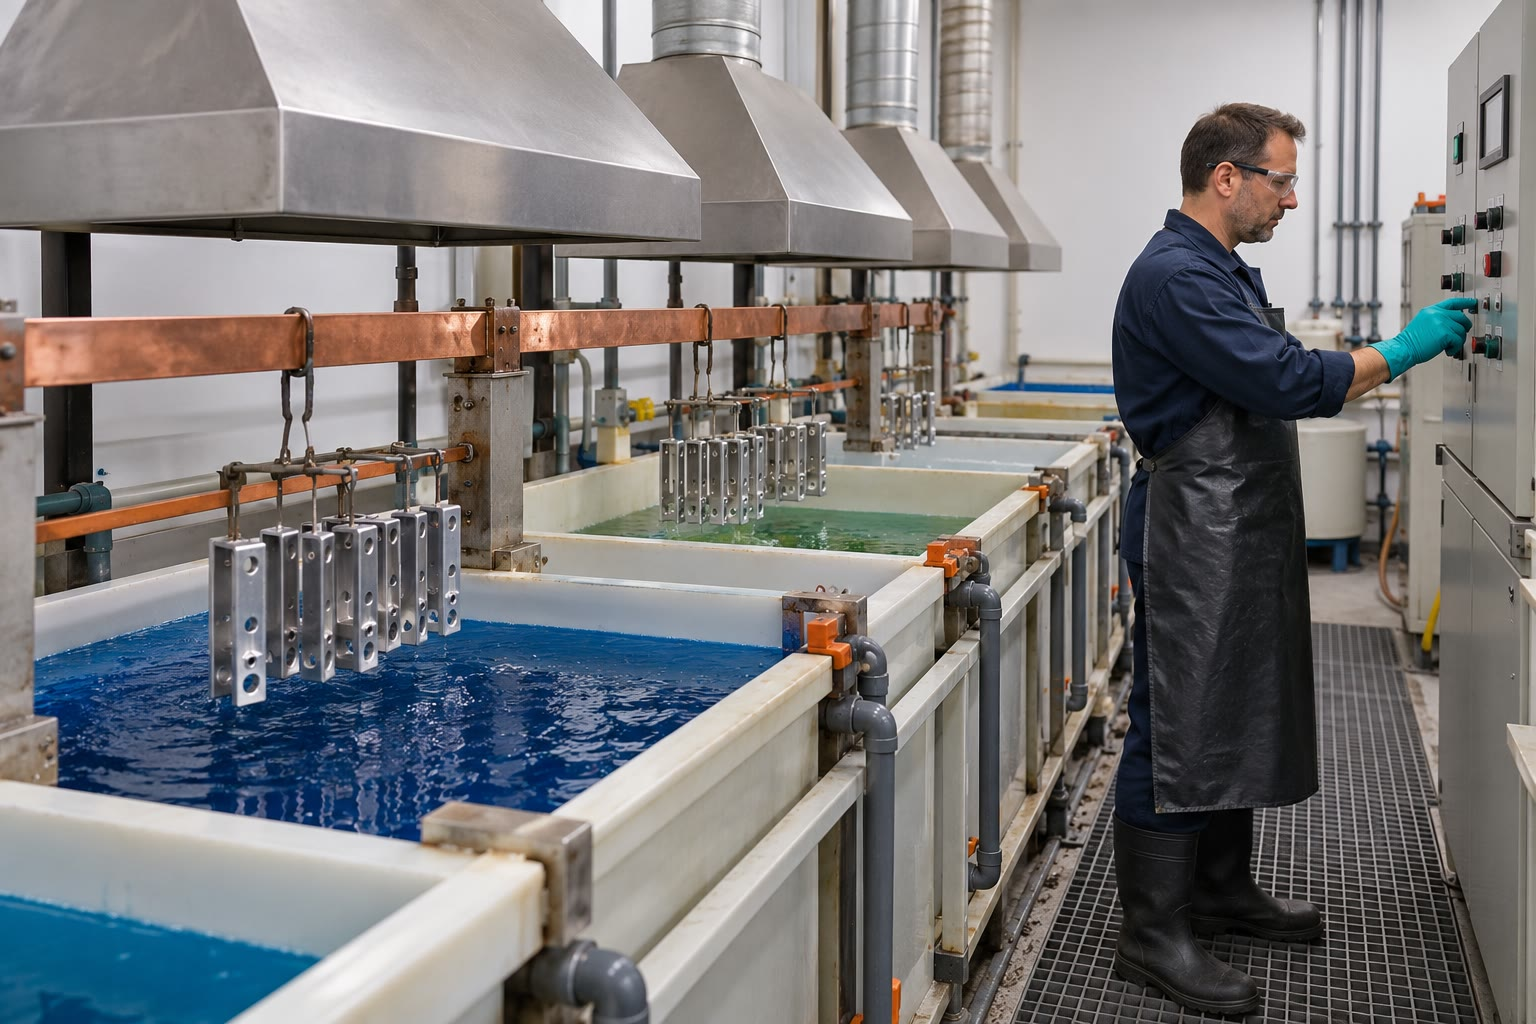
\includegraphics[width=0.62\linewidth]{images/book3/ai/b2-10-electroplating.jpg}

{\small Uma linha de galvanoplastia: as peças a revestir pendem de barramentos
de cobre dentro dos banhos e são ligadas como cátodo; o operador ajusta a
corrente no retificador. A corrente fixa a velocidade com que o metal se
deposita; o potencial das peças decide qual metal, ou quanto hidrogênio, se
forma junto.}
\end{omfigure}

\section{Um eletrodo fora do equilíbrio}

\begin{definition}[Curva corrente--potencial]\label{def:b2:current-potential-curves:ie-curve}
A \emph{curva corrente--potencial}\index{curva corrente--potencial} de um
eletrodo em uma solução é o gráfico da corrente $i$ que atravessa o eletrodo
em função de seu potencial $E$. Uma \emph{corrente anódica}\index{corrente anodica@corrente anódica},
contada positivamente, corresponde a uma oxidação no eletrodo; uma
\emph{corrente catódica}\index{corrente catodica@corrente catódica}, contada negativamente, a uma
redução.
\end{definition}

\begin{definition}[Espécie eletroativa]\label{def:b2:current-potential-curves:electroactive}
Uma \emph{espécie eletroativa}\index{especie eletroativa@espécie eletroativa} é uma espécie
que pode ser oxidada ou reduzida no eletrodo na faixa de potenciais
considerada.
\end{definition}

\begin{proposition}[Corrente e velocidade]\label{prop:b2:current-potential-curves:current-rate}
Se uma única semirreação com $n$ elétrons ocorre em um eletrodo, a
corrente mede sua velocidade: $i = nF\,d\xi/dt$, sendo $\xi$ o avanço
da oxidação (de modo que $i > 0$ para uma oxidação e $i < 0$ para uma redução).
\end{proposition}

\begin{proof}
Pela \cref{prop:b2:cell-thermodynamics:charge}, um avanço $d\xi$ faz passar a
carga $nF\,d\xi$ pelo eletrodo no tempo $dt$.
\end{proof}

Para registrar uma tal curva, é preciso impor e medir o potencial de um
eletrodo enquanto uma corrente o atravessa --- o que uma montagem de dois
eletrodos não consegue fazer, já que a corrente também muda o potencial do
segundo eletrodo.

\begin{definition}[Montagem de três eletrodos]\label{def:b2:current-potential-curves:set-up}
Em uma montagem de três eletrodos, a corrente circula entre o \emph{eletrodo
de trabalho}\index{eletrodo de trabalho}, o que é estudado, e o \emph{contraeletrodo}\index{contraeletrodo},
que fecha o circuito; o potencial do eletrodo de
trabalho é medido em relação a um eletrodo de referência pelo qual não
passa corrente. Um potenciostato eletrônico ajusta a corrente para que esse
potencial mantenha o valor imposto.
\end{definition}

\begin{omfigure}
\begin{tikzpicture}[font=\small, >={Stealth}]
  \pic[transform shape] at (0,0) {beaker={0.7}{omDef!14}};
  \pic at (-0.55,0.25) {electrode={black!35}};
  \pic at (0.55,0.25) {electrode={black!15}};
  \pic (r) at (0.0,0.15) {probe};
  \draw[thick, rounded corners] (-2.2,4.3) rectangle (2.2,5.5);
  \node at (0,4.9) {potenciostato};
  \draw[thick, omThm] (-0.40,2.65) -- (-0.40,3.5) -- (-1.6,3.5) -- (-1.6,4.3);
  \draw[thick, omDef] (0.70,2.65) -- (0.70,3.5) -- (1.6,3.5) -- (1.6,4.3);
  \draw[thick] (r-top) -- (0,4.3);
  \node[anchor=east, font=\scriptsize, omThm] at (-1.65,3.85) {ET};
  \node[anchor=west, font=\scriptsize, omDef] at (1.65,3.85) {CE};
  \node[anchor=west, font=\scriptsize] at (0.05,3.95) {ER};
  \draw[<-, omProp, thick] (-0.75,1.2) -- (-2.0,1.4) node[left, text=black, align=right] {eletrodo\\ de trabalho};
  \draw[<-, omProp, thick] (0.85,1.2) -- (2.1,1.4) node[right, text=black, align=left] {contra-\\eletrodo};
  \draw[<-, omProp, thick] (0.05,0.5) -- (1.4,-0.4) node[right, text=black] {eletrodo de referência};
  \node[font=\scriptsize, align=center] at (0,6.0) {impõe $E_{\text{ET}} - E_{\text{ER}}$, mede $i$};
\end{tikzpicture}

{\small A montagem de três eletrodos. O potenciostato impõe a corrente entre o
\omterm{def:b2:current-potential-curves:set-up}{eletrodo de trabalho} (ET) e o \omterm{def:b2:current-potential-curves:set-up}{contraeletrodo} (CE) de modo a manter o
potencial do \omterm{def:b2:current-potential-curves:set-up}{eletrodo de trabalho}, medido em relação ao eletrodo de
referência (ER), no valor imposto; nenhuma corrente passa pela
referência.}
\end{omfigure}

Quando não circula corrente e as duas formas de um par estão presentes, o
eletrodo assume o potencial de Nernst do par --- se a troca de elétrons for
rápida o bastante para estabelecê-lo. Afastar o potencial desse valor faz
circular uma corrente.

\section{Sistemas rápidos e lentos}

\begin{definition}[Sobretensão]\label{def:b2:current-potential-curves:overpotential}
A \emph{sobretensão}\index{sobretensao@sobretensão} de um eletrodo atravessado por uma
corrente $i$ é $\eta = E(i) - E_{\text{eq}}$, a diferença entre seu
potencial e o potencial de equilíbrio (de Nernst) do par. O
\emph{potencial de limiar}\index{potencial de limiar} de uma semirreação é o
potencial além do qual sua corrente se torna apreciável.
\end{definition}

\begin{definition}[Sistemas rápidos e lentos]\label{def:b2:current-potential-curves:fast-slow}
Um par é um \emph{sistema rápido}\index{sistema rapido@sistema rápido} em um dado eletrodo se
uma corrente apreciável circula assim que o potencial se afasta de seu
potencial de Nernst; é um \emph{sistema lento}\index{sistema lento} se é
necessária uma \omterm{def:b2:current-potential-curves:overpotential}{sobretensão} de alguns décimos de volt antes que a corrente se
torne apreciável, em um sentido ou no outro.
\end{definition}

Um sistema ser rápido ou lento depende do par e do material do eletrodo. Os
pares \ce{Fe^3+}/\ce{Fe^2+} e \ce{Ag+}/\ce{Ag} são rápidos sobre a platina; a
redução de \ce{H+} é rápida sobre a platina, mas lenta sobre o mercúrio, o
chumbo ou o zinco; a oxidação da água a dioxigênio é lenta sobre qualquer
eletrodo. As transferências de elétrons que rompem ou formam ligações, como as
de \ce{O2} ou de \ce{H2}, são tipicamente lentas; a transferência de um elétron
entre dois íons de forma quase igual é rápida. A forma da parte ascendente
de uma curva lenta vem da cinética da transferência eletrônica, deduzida no
volume do 3.º ano.

\begin{omfigure}
\begin{tikzpicture}
\begin{axis}[omie, width=0.47\linewidth, height=5.4cm, xmin=0.25, xmax=1.3,
  ymin=-1.3, ymax=1.3, xlabel={$E$}, ylabel={$i$}, title={\small sistema rápido}]
\addplot[omanodic] table[x=E, y=i, restrict expr to domain={\thisrow{i}}{0:2}] {figdata/out/bachelor-2-ie-curves-a.dat};
\addplot[omcathodic] table[x=E, y=i, restrict expr to domain={\thisrow{i}}{-2:0}] {figdata/out/bachelor-2-ie-curves-a.dat};
\draw[densely dotted] (axis cs:0.77,-1.2) -- (axis cs:0.77,1.2);
\node[font=\scriptsize, anchor=north west] at (axis cs:0.78,-0.05) {$E_{\text{eq}}$};
\node[font=\scriptsize, anchor=south] at (axis cs:1.1,1.0) {\ce{Fe^2+} $\to$ \ce{Fe^3+}};
\node[font=\scriptsize, anchor=north] at (axis cs:0.45,-1.0) {\ce{Fe^3+} $\to$ \ce{Fe^2+}};
\end{axis}
\end{tikzpicture}\hfill
\begin{tikzpicture}
\begin{axis}[omie, width=0.47\linewidth, height=5.4cm, xmin=-0.25, xmax=1.8,
  ymin=-1.3, ymax=1.3, xlabel={$E$}, ylabel={$i$}, title={\small sistema lento}]
\addplot[omanodic] table[x=E, y=i, restrict expr to domain={\thisrow{i}}{0:2}] {figdata/out/bachelor-2-ie-curves-c.dat};
\addplot[omcathodic] table[x=E, y=i, restrict expr to domain={\thisrow{i}}{-2:0}] {figdata/out/bachelor-2-ie-curves-c.dat};
\draw[densely dotted] (axis cs:0.77,-1.2) -- (axis cs:0.77,1.2);
\draw[<->, omProp] (axis cs:0.77,0.5) -- (axis cs:1.12,0.5) node[midway, above, font=\scriptsize] {$\eta_a$};
\draw[<->, omProp] (axis cs:0.42,-0.5) -- (axis cs:0.77,-0.5) node[midway, below, font=\scriptsize] {$\eta_c$};
\node[font=\scriptsize, anchor=north west] at (axis cs:0.78,-0.05) {$E_{\text{eq}}$};
\end{axis}
\end{tikzpicture}

{\small \omterm{def:b2:current-potential-curves:ie-curve}{Curvas corrente--potencial} modelo de um par cujas duas formas estão
presentes em concentrações iguais (ramo anódico em vermelho, catódico em
azul). À esquerda, um \omterm{def:b2:current-potential-curves:fast-slow}{sistema rápido}: a corrente muda de sinal abruptamente no
potencial de equilíbrio. À direita, um \omterm{def:b2:current-potential-curves:fast-slow}{sistema lento}: nenhuma corrente
circula em uma faixa de potenciais em torno dele; cada ramo exige uma
\omterm{def:b2:current-potential-curves:overpotential}{sobretensão}. Ambos atingem os mesmos patamares limite, fixados pela difusão.
(Valores ilustrativos.)}
\end{omfigure}

\section{Transporte de matéria e correntes limite}

Quando a transferência de elétrons é rápida, a corrente é limitada pela
chegada do reagente ao eletrodo. Em uma solução agitada, uma fina camada de
líquido junto ao eletrodo fica quase imóvel, e o reagente a atravessa por
difusão.

\begin{definition}[Camada de difusão e corrente limite]\label{def:b2:current-potential-curves:limiting-current}
A \emph{camada de difusão}\index{camada de difusao@camada de difusão} é a camada de solução,
de espessura $\delta$ (de alguns a algumas dezenas de micrômetros em uma
solução agitada), junto ao eletrodo, através da qual as espécies se deslocam
apenas por difusão. A \emph{corrente limite}\index{corrente limite} é a corrente
atingida quando a \omterm{def:b2:current-potential-curves:electroactive}{espécie eletroativa} é consumida tão depressa quanto chega,
sendo nula sua concentração na superfície.
\end{definition}

\begin{omfigure}
\begin{tikzpicture}[font=\small, >={Stealth}, x=1.2cm, y=1.2cm]
  \fill[black!25] (-0.4,0) rectangle (0,3);
  \node[rotate=90, font=\scriptsize] at (-0.2,1.5) {eletrodo};
  \draw[->] (0,0) -- (4.6,0) node[right] {$x$};
  \draw[->] (0,0) -- (0,3.2) node[above] {$c$};
  \draw[densely dashed] (1.6,0) -- (1.6,3);
  \node[below, font=\scriptsize] at (1.6,0) {$\delta$};
  \draw[omDef, thick] (0,1.2) -- (1.6,2.4) -- (4.4,2.4);
  \draw[omThm, thick] (0,0.02) -- (1.6,2.4);
  \node[font=\scriptsize, anchor=west] at (2.6,2.6) {seio da solução, $c^b$ (agitado)};
  \node[font=\scriptsize, omDef, anchor=east] at (-0.45,1.2) {$c^s$};
  \node[font=\scriptsize, omThm, anchor=west] at (1.7,0.5) {$c^s = 0$: corrente limite};
  \node[font=\scriptsize, align=center] at (0.8,3.0) {camada de\\ difusão};
\end{tikzpicture}

{\small Concentração do reagente perto de um eletrodo em uma solução
agitada. Através da \omterm{def:b2:current-potential-curves:limiting-current}{camada de difusão} o perfil é linear; o fluxo, e portanto a
corrente, é proporcional a $c^b - c^s$. Ele é máximo quando o reagente é
consumido assim que chega ($c^s = 0$, em vermelho).}
\end{omfigure}

\begin{theorem}[Corrente limite]\label{thm:b2:current-potential-curves:limiting}
Para uma espécie de concentração $c$ no seio da solução e coeficiente de
difusão $D$, que atravessa uma \omterm{def:b2:current-potential-curves:limiting-current}{camada de difusão} de espessura $\delta$ até
um eletrodo de área $A$, a \omterm{def:b2:current-potential-curves:limiting-current}{corrente limite} é, em valor absoluto,
\[
  |i_{\lim}| = \frac{nFADc}{\delta} .
\]
\end{theorem}

\begin{proof}
Em regime estacionário, o perfil de concentração na camada é linear (a segunda
lei de Fick com $\partial c/\partial t = 0$ dá $d^2c/dx^2 = 0$); logo o fluxo
em direção ao eletrodo é $j = D(c - c^s)/\delta$, em mols por unidade de área e
de tempo. Cada molécula que chega reage com $n$ elétrons: $|i| = nFAj =
nFAD(c - c^s)/\delta$, máximo para $c^s = 0$.
\end{proof}

\begin{example}[Ordem de grandeza de uma corrente limite]\label{ex:b2:current-potential-curves:ilim}
Para uma espécie a \qty{10}{mmol/L} (\qty{10}{mol/m^3}), com $D =
\qty{7e-10}{m^2/s}$, $\delta = \qty{20}{\micro m}$, $n = 1$, sobre
\qty{1.0}{cm^2}: $|i_{\lim}| = 96\,485 \times 10^{-4} \times 7 \times 10^{-10}
\times 10/(2 \times 10^{-5}) = \qty{3.4}{mA}$.
\end{example}

\begin{theorem}[Onda de um sistema rápido]\label{thm:b2:current-potential-curves:wave}
Para um par rápido $\mathrm{Ox} + n\,\mathrm e^- \rightleftharpoons \mathrm{Red}$,
com \omterm{def:b2:current-potential-curves:limiting-current}{corrente limite} anódica $i_{\lim,a} > 0$ (fixada por Red) e \omterm{def:b2:current-potential-curves:limiting-current}{corrente
limite} catódica $i_{\lim,c} < 0$ (fixada por Ox), a curva estacionária é
\[
  E = E_{1/2} + \frac{RT}{nF}\ln\frac{i - i_{\lim,c}}{i_{\lim,a} - i},
  \qquad E_{1/2} = E^\circ + \frac{RT}{nF}\ln\frac{D_{\text{Red}}}{D_{\text{Ox}}} ,
\]
sendo a espessura da camada a mesma para as duas formas.
\end{theorem}

\begin{proof}
Para um \omterm{def:b2:current-potential-curves:fast-slow}{sistema rápido}, a equação de Nernst vale na superfície do eletrodo, $E = E^\circ + (RT/nF)
\ln(c^s_{\text{Ox}}/c^s_{\text{Red}})$. Perfis lineares: uma \omterm{def:b2:current-potential-curves:ie-curve}{corrente anódica} $i$
consome Red e produz Ox na superfície, $i = nFAD_{\text{Red}}(c^b_{\text{Red}}
- c^s_{\text{Red}})/\delta = -nFAD_{\text{Ox}}(c^b_{\text{Ox}} - c^s_{\text{Ox}})/\delta$.
Com $i_{\lim,a} = nFAD_{\text{Red}}c^b_{\text{Red}}/\delta$ e $i_{\lim,c} =
-nFAD_{\text{Ox}}c^b_{\text{Ox}}/\delta$, essas relações dão $c^s_{\text{Red}} = (i_{\lim,a} -
i)\delta/(nFAD_{\text{Red}})$ e $c^s_{\text{Ox}} = (i - i_{\lim,c})\delta/(nFAD_{\text{Ox}})$.
Substitua na equação de Nernst.
\end{proof}

\begin{corollary}[Potencial de meia-onda]\label{cor:b2:current-potential-curves:half-wave}
Quando as duas formas têm coeficientes de difusão iguais, $E_{1/2} = E^\circ$:
com uma só forma presente, a corrente vale metade de seu valor limite no
potencial padrão do par.
\end{corollary}

\begin{proof}
Com apenas Red presente, $i_{\lim,c} = 0$, e para $i = i_{\lim,a}/2$ o logaritmo
se anula: $E = E_{1/2} = E^\circ$ quando $D_{\text{Red}} = D_{\text{Ox}}$.
\end{proof}

\begin{proposition}[Os patamares medem concentrações]\label{prop:b2:current-potential-curves:plateau}
Com agitação e eletrodo fixos, a altura de um patamar é proporcional à
concentração da espécie que ele consome: um eletrodo mantido em um
potencial do patamar é um sensor amperométrico.
\end{proposition}

\begin{proof}
$|i_{\lim}| = (nFAD/\delta)\,c$, e o fator entre parênteses é constante com
agitação e temperatura fixas.
\end{proof}

\begin{omfigure}
\begin{tikzpicture}
\begin{axis}[omie, width=0.47\linewidth, height=5.0cm, xmin=0.25, xmax=1.3,
  ymin=-0.3, ymax=1.3, xlabel={$E$}, ylabel={$i$}, title={\small só \ce{Fe^2+} presente}]
\addplot[omanodic] table[x=E, y=i] {figdata/out/bachelor-2-ie-curves-b.dat};
\draw[densely dotted] (axis cs:0.77,0) -- (axis cs:0.77,0.5) -- (axis cs:0.25,0.5);
\node[font=\scriptsize, anchor=north] at (axis cs:0.77,-0.02) {$E_{1/2}$};
\node[font=\scriptsize, anchor=south west] at (axis cs:0.27,0.5) {$i_{\lim}/2$};
\node[font=\scriptsize, anchor=south] at (axis cs:1.12,1.0) {patamar};
\end{axis}
\end{tikzpicture}\hfill
\begin{tikzpicture}
\begin{axis}[width=0.42\linewidth, height=5.0cm, xmin=0, xmax=1.05, ymin=0, ymax=1.1,
  axis x line=bottom, axis y line=left, xtick=\empty, ytick=\empty,
  xlabel={$c$}, ylabel={$i_{\lim}$}, label style={font=\small},
  title={\small amperometria}]
\addplot[omanodic, mark=*, mark size=1.2pt] table[x=c, y=i] {figdata/out/bachelor-2-ie-curves-e.dat};
\end{axis}
\end{tikzpicture}

{\small À esquerda: a onda de um par rápido quando só a forma reduzida está
presente (modelo); sua meia-altura fica no potencial de meia-onda. À direita:
a altura do patamar cresce proporcionalmente à concentração.}
\end{omfigure}

\section{O solvente e o eletrodo}

A própria água é eletroativa: ela é oxidada a dioxigênio
(\ce{2H2O -> O2 + 4H+ + 4e-}) e reduzida a di-hidrogênio (\ce{2H+ + 2e- -> H2}, ou
\ce{2H2O + 2e- -> H2 + 2OH-}). Como o solvente nunca se esgota, suas curvas
não têm patamar: elas sobem abruptamente e limitam todas as outras curvas.

\begin{definition}[Janela de eletroatividade]\label{def:b2:current-potential-curves:window}
As \emph{barreiras do solvente}\index{barreira do solvente} são os ramos abruptos da
oxidação e da redução do solvente. A \emph{janela de
eletroatividade}\index{janela de eletroatividade} é a faixa de potenciais entre elas,
na qual as curvas das espécies dissolvidas podem ser observadas.
\end{definition}

\begin{proposition}[A janela da água]\label{prop:b2:current-potential-curves:window}
Na água, a um dado pH, a janela fica em torno da faixa termodinâmica dos
dois pares da água, $\qty{0}{V} - 0.059\,\mathrm{pH}$ e $\qty{1.23}{V} -
0.059\,\mathrm{pH}$, alargada de cada lado pela \omterm{def:b2:current-potential-curves:overpotential}{sobretensão} da reação
correspondente no eletrodo usado.
\end{proposition}

\begin{proof}[Raciocínio]
Cada barreira começa perto do potencial de Nernst de seu par, deslocado pela
\omterm{def:b2:current-potential-curves:overpotential}{sobretensão} de limiar: a oxidação da água é lenta sobre todos os eletrodos;
por isso a barreira anódica fica alguns décimos de volt acima de \qty{1.23}{V}
(a pH 0); a redução de \ce{H+} é rápida sobre a platina, cuja barreira
catódica fica perto de \qty{0}{V}, mas lenta sobre o zinco, o chumbo ou o
mercúrio, cuja barreira fica vários décimos de volt mais abaixo.
\end{proof}

\begin{omfigure}
\begin{tikzpicture}
\begin{axis}[omie, width=0.82\linewidth, height=5.4cm, xmin=-1.2, xmax=2.0,
  ymin=-3, ymax=3, xlabel={$E$ (V)}, ylabel={$i$}, clip=true, clip mode=individual]
\addplot[omwall] table[x=E, y=i] {figdata/out/bachelor-2-ie-curves-d-high.dat};
\addplot[omcathodic] table[x=E, y=i, restrict expr to domain={\thisrow{E}}{-1.2:0.6}] {figdata/out/bachelor-2-ie-curves-d-Pt.dat};
\addplot[omanodic] table[x=E, y=i, restrict expr to domain={\thisrow{E}}{0.6:2.0}] {figdata/out/bachelor-2-ie-curves-d-Pt.dat};
\draw[densely dotted] (axis cs:0,-2.8) -- (axis cs:0,2.8);
\draw[densely dotted] (axis cs:1.23,-2.8) -- (axis cs:1.23,2.8);
\node[font=\scriptsize, anchor=north west] at (axis cs:0.02,-0.1) {0};
\node[font=\scriptsize, anchor=north west] at (axis cs:1.24,-0.1) {1.23};
\node[font=\scriptsize, omDef, anchor=west] at (axis cs:0.05,-2.2) {\ce{H+} $\to$ \ce{H2} sobre Pt};
\node[font=\scriptsize, gray, anchor=east] at (axis cs:-0.85,-1.0) {sobre Zn, Pb};
\node[font=\scriptsize, omThm, anchor=east] at (axis cs:1.18,2.2) {\ce{H2O} $\to$ \ce{O2}};
\end{axis}
\end{tikzpicture}

{\small As barreiras da água a pH 0 (modelo). A redução de \ce{H+} começa perto
de \qty{0}{V} sobre a platina (em azul), mas vários décimos de volt mais abaixo
sobre metais como o zinco ou o chumbo (tracejado); a oxidação da água exige uma
\omterm{def:b2:current-potential-curves:overpotential}{sobretensão} sobre qualquer eletrodo. A janela é a faixa entre as barreiras.}
\end{omfigure}

\section{Ler as curvas}

\begin{method}[Esboçar as curvas de uma solução]\label{met:b2:current-potential-curves:sketch-ie}
\begin{enumerate}
  \item Trace as duas \omterm{def:b2:current-potential-curves:window}{barreiras do solvente} para o pH e o material do
        eletrodo.
  \item Para cada par presente, situe seu potencial de Nernst (as duas formas
        presentes) ou $E^\circ$ (uma forma): um \omterm{def:b2:current-potential-curves:fast-slow}{sistema rápido} corta o eixo ali
        abruptamente; um \omterm{def:b2:current-potential-curves:fast-slow}{sistema lento} é deslocado por suas \omterm{def:b2:current-potential-curves:overpotential}{sobretensões}.
  \item Dê a cada onda um patamar proporcional à concentração da espécie que
        ela consome; um eletrodo metálico que se oxida a si mesmo não tem
        patamar (o metal não se esgota).
  \item Some as correntes das reações possíveis em cada potencial.
\end{enumerate}
\end{method}

\begin{method}[Ler as curvas]\label{met:b2:current-potential-curves:read-ie}
\begin{enumerate}
  \item A potencial imposto, leia em cada curva a corrente de cada reação:
        elas ocorrem simultaneamente, na proporção de suas correntes.
  \item A corrente imposta (eletrólise), encontre o potencial no qual as
        curvas anódicas ou catódicas somam essa corrente; as reações envolvidas
        são aquelas cujas curvas contribuem ali.
  \item Para uma pilha, ou um metal que sofre corrosão, a \omterm{def:b2:current-potential-curves:ie-curve}{corrente anódica} de
        uma reação é igual à \omterm{def:b2:current-potential-curves:ie-curve}{corrente catódica} da outra: procure esse par de
        pontos.
\end{enumerate}
\end{method}

\begin{example}[Zincagem a partir de um banho ácido]\label{ex:b2:current-potential-curves:zinc}
Em um banho ácido de zinco, o cátodo admite duas reduções possíveis: \ce{Zn^2+
+ 2e- -> Zn} ($E^\circ = \qty{-0.76}{V}$, rápida) e \ce{2H+ + 2e- -> H2}
($E^\circ = \qty{0}{V}$). Termodinamicamente, o hidrogênio deveria vir primeiro
e o zinco nunca. Mas sobre o zinco a redução de \ce{H+} é lenta: sua barreira
fica abaixo de \qty{-0.76}{V} e, no potencial em que o zinco se deposita a uma
velocidade útil, forma-se pouco hidrogênio. É a curva, e não o diagrama, que
explica o revestimento.
\end{example}

\begin{history}[A polarografia]
\begin{minipage}[t]{0.25\linewidth}
\vspace{0pt}
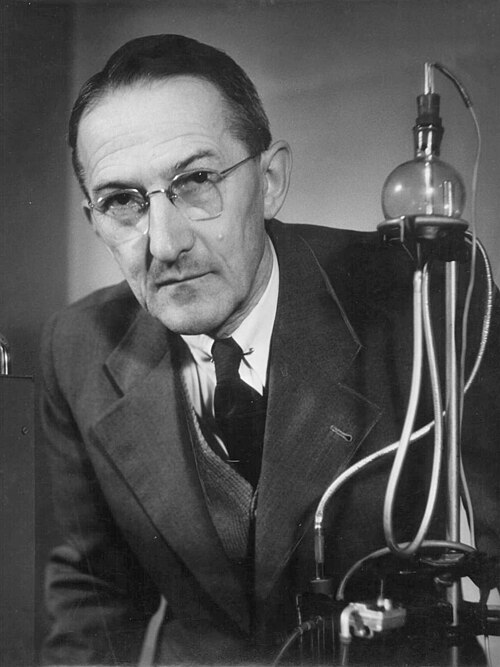
\includegraphics[width=\linewidth]{images/book3/heyrovsky.jpg}
\end{minipage}\hfill
\begin{minipage}[t]{0.71\linewidth}
\vspace{0pt}
Em 1922, Jaroslav Heyrovský registrou a corrente através de um eletrodo de
mercúrio que se formava gota a gota na ponta de um capilar, enquanto o
potencial era varrido: cada espécie redutível dava um degrau cuja posição a
identificava e cuja altura media sua concentração. A gota renovada mantinha a
superfície limpa, e a alta \omterm{def:b2:current-potential-curves:overpotential}{sobretensão} do hidrogênio sobre o mercúrio abria
uma ampla janela catódica. A polarografia lhe valeu o Prêmio Nobel de Química
em 1959 e fundou a química eletroanalítica; a fotografia o mostra com um
eletrodo gotejante de mercúrio. (Fotografia: arquivo do Instituto J.~Heyrovský
de Físico-Química, CC BY-SA 3.0, Wikimedia Commons.)
\end{minipage}
\end{history}

\section{Exercícios}

\begin{exercise}[$\star$]\label{exo:b2:current-potential-curves:1}
Em uma pilha de Daniell que fornece corrente, dê o sinal da corrente no
eletrodo de zinco e no eletrodo de cobre, com as convenções deste
capítulo.
\end{exercise}

\begin{exercise}[$\star$]\label{exo:b2:current-potential-curves:2}
Calcule a \omterm{def:b2:current-potential-curves:limiting-current}{corrente limite} da redução de \ce{Ag+} (\qty{2.0}{mmol/L}, $D =
\qty{1.6e-9}{m^2/s}$) sobre \qty{0.50}{cm^2} com $\delta = \qty{25}{\micro m}$
(valores de modelo).
\end{exercise}

\begin{exercise}[$\star$]\label{exo:b2:current-potential-curves:3}
Nas curvas modelo do capítulo, como se reconhece um \omterm{def:b2:current-potential-curves:fast-slow}{sistema rápido} e um
\omterm{def:b2:current-potential-curves:fast-slow}{sistema lento}? Dê um exemplo de cada um sobre a platina.
\end{exercise}

\begin{exercise}[$\star$]\label{exo:b2:current-potential-curves:4}
Uma solução contém apenas \ce{Fe^2+}. Em que potencial sua \omterm{def:b2:current-potential-curves:ie-curve}{corrente anódica}
atinge a metade de seu patamar, se as duas formas difundem do mesmo modo ($E^\circ = \qty{0.77}{V}$)?
\end{exercise}

\begin{exercise}[$\star\star$]\label{exo:b2:current-potential-curves:5}
Um eletrodo de platina em uma solução de \ce{Fe^3+} e \ce{Cu^2+} (concentrações
iguais, $E^\circ$ = 0.77 e \qty{0.34}{V}) é varrido em direção a potenciais
negativos. Descreva a curva: ondas, patamares, suas alturas e a barreira
catódica.
\end{exercise}

\begin{exercise}[$\star\star$]\label{exo:b2:current-potential-curves:6}
Na solução do \cref{exo:b2:current-potential-curves:5}, o potencial do
eletrodo é mantido em \qty{0.50}{V} e depois em \qty{0.10}{V}. O que acontece
em cada caso?
\end{exercise}

\begin{exercise}[$\star\star$]\label{exo:b2:current-potential-curves:7}
Dê os potenciais de Nernst dos dois pares da água a pH 0 e a pH 14, e
esboce como a janela sobre a platina se desloca com o pH.
\end{exercise}

\begin{exercise}[$\star\star$]\label{exo:b2:current-potential-curves:8}
O \ce{Fe^2+} é titulado pelo \ce{Ce^4+} enquanto um eletrodo de platina
mantido em \qty{1.0}{V} registra a corrente. Esboce a corrente em função do
volume adicionado e explique como ela localiza a equivalência (\ce{Ce^4+}/\ce{Ce^3+}: $E^\circ =
\qty{1.72}{V}$).
\end{exercise}

\begin{exercise}[$\star\star$]\label{exo:b2:current-potential-curves:9}
Dobrar a velocidade de agitação divide por dois a espessura da \omterm{def:b2:current-potential-curves:limiting-current}{camada de
difusão}. O que acontece com os patamares, com o potencial de meia-onda e com
o potencial de corrente nula de um \omterm{def:b2:current-potential-curves:fast-slow}{sistema rápido}?
\end{exercise}

\begin{exercise}[$\star\star\star$]\label{exo:b2:current-potential-curves:10}
Deduza a equação da onda de um \omterm{def:b2:current-potential-curves:fast-slow}{sistema rápido} com apenas Red presente e
mostre que um gráfico de $E$ em função de $\log[i/(i_{\lim} - i)]$ é uma reta
de inclinação $0.059/n$ volt a \qty{25}{\degreeCelsius}.
\end{exercise}

\begin{exercise}[$\star\star\star$]\label{exo:b2:current-potential-curves:11}
Um pedaço de zinco mergulhado em ácido a \qty{1}{mol/L} se dissolve apenas
lentamente, enquanto o mesmo pedaço em contato com um fio de platina se
dissolve depressa, com hidrogênio borbulhando sobre a platina. Explique com
\omterm{def:b2:current-potential-curves:ie-curve}{curvas corrente--potencial}.
\end{exercise}

\begin{exercise}[$\star\star\star$]\label{exo:b2:current-potential-curves:12}
Para oxidar uma espécie cuja onda fica em \qty{2.0}{V} a pH 0, você escolheria
um eletrodo de platina ou um eletrodo com alta \omterm{def:b2:current-potential-curves:overpotential}{sobretensão} de oxigênio?
Explique e diga o que se formaria caso contrário.
\end{exercise}

\section{Problema: Uma sonda de oxigênio para um rio}

\begin{problem}[{Problema de fim de semana --- o cátodo de um sensor
amperométrico de oxigênio, a corrente limite através de sua membrana, a
calibração em água saturada de ar com a lei de Henry e o teor de oxigênio
de um rio}]
\label{pb:b2:current-potential-curves:1}
Uma sonda amperométrica de oxigênio tem um cátodo de ouro e um ânodo de prata
em um gel de cloreto de potássio, separados da amostra por uma fina membrana
permeável a gases. O cátodo é mantido em \qty{-0.60}{V} em relação ao ânodo de
prata--cloreto de prata. Dados a \qty{25}{\degreeCelsius}: constante da \omterm{prop:b2:chemical-potential:henry}{lei de
Henry} do \ce{O2}, $H = \qty{1.3e-5}{mol/(m^3.Pa)}$; pressão de vapor da água
\qty{3.17}{kPa}; oxigênio no ar seco 20.95~\% em volume; $E^\circ(\ce{O2}/\ce{H2O}) =
\qty{1.229}{V}$; $E^\circ(\ce{AgCl}/\ce{Ag}) = \qty{0.222}{V}$. Membrana (valores
de modelo): área \qty{0.10}{cm^2}, espessura \qty{25}{\micro m}, coeficiente de
difusão efetivo do \ce{O2} através dela \qty{1.0e-10}{m^2/s}.
% ledger: henry:O2, pvap:H2O.298, air:O2, dfg:Cl-_ao, dfg:AgCl_cr, aw:O

\medskip
\noindent\textbf{Parte I --- O cátodo.}
\begin{enumerate}
  \item Escreva a redução do dioxigênio em meio neutro.
  \item Escreva a reação no ânodo de prata e a reação global.
  \item Calcule o potencial de Nernst do par \ce{O2}/\ce{H2O} a pH 7 com
        $p_{\ce{O2}} = \qty{0.21}{bar}$.
  \item Expresse o potencial do cátodo, \qty{-0.60}{V} em relação a Ag/AgCl,
        na escala do hidrogênio, tomando como 1 a atividade do cloreto no gel.
  \item Por que o cátodo deve ser mantido muito abaixo do potencial de Nernst
        do \ce{O2}?
  \item Por que se escolhe um potencial no patamar?
  \item O que fixa o limite inferior dos potenciais utilizáveis?
\end{enumerate}

\medskip
\noindent\textbf{Parte II --- A \omterm{def:b2:current-potential-curves:limiting-current}{corrente limite}.}
\begin{enumerate}[resume]
  \item Descreva o perfil de concentração do \ce{O2} através da membrana quando o
        cátodo funciona em seu patamar.
  \item Escreva o fluxo de \ce{O2} através da membrana.
  \item Deduza a corrente em função da concentração $c$ de \ce{O2}
        dissolvido.
  \item Por que se usa a espessura da membrana no lugar da \omterm{def:b2:current-potential-curves:limiting-current}{camada de difusão}?
  \item Por que a leitura depende pouco da agitação do rio, mas muito da
        incrustação da membrana?
\end{enumerate}

\medskip
\noindent\textbf{Parte III --- A calibração.}
\begin{enumerate}[resume]
  \item Calcule a pressão parcial do \ce{O2} sobre a água saturada de ar a
        \qty{1.013}{bar} e \qty{25}{\degreeCelsius}.
  \item Calcule a concentração de \ce{O2} dissolvido na saturação, em
        \unit{mol/m^3}.
  \item Expresse-a em \unit{mg/L}.
  \item Preveja a corrente da sonda em água saturada de ar.
  \item A sonda lê de fato \qty{4.05}{\micro A} em água saturada de ar
        (dados do exercício). Calcule sua sensibilidade em \unit{\micro A} por
        \unit{mg/L}.
  \item Por que calibrar em vez de confiar na corrente prevista?
  \item O que a sonda deveria ler em água isenta de oxigênio?
\end{enumerate}

\medskip
\noindent\textbf{Parte IV --- O rio.}
\begin{enumerate}[resume]
  \item Em uma amostra de rio a \qty{25}{\degreeCelsius}, a sonda lê
        \qty{2.80}{\micro A}. Calcule o oxigênio dissolvido em \unit{mg/L}.
  \item Expresse-o como porcentagem da saturação.
  \item A água de um rio está quase saturada de oxigênio na nascente.
        Sugira uma causa para o déficit.
  \item Que quantidade de \ce{O2} a sonda consome em uma hora? Ela perturba
        a amostra?
  \item Por que a calibração deve ser refeita se o rio estiver a
        \qty{15}{\degreeCelsius}?
  \item Dê a concentração de oxigênio dissolvido da amostra.
\end{enumerate}
\end{problem}
